\newpage
	\section{Задачи для подготовки к контрольной 1}
		\subsection{ПК1 1}
		A)\\
		Прямые -
		\begin{gather*}
		a: 28x_1 - 4x_2 = 16 \\
		b: -13x_1 + 2x_2 = -8 \\
		c: -41x_1 + 6x_2 = -20 
		\end{gather*}
		Пусть точки $A$, $B$ и $C$ - $b \cap c$, $c \cap a$ и $a \cap b$ соотв. Тогда -
		\begin{gather*}
		A:\\
		-13x_1 + 2x_2 = -8 \Longleftrightarrow 2x_2 = -8 + 13x_1 \\
		-41x_1 + 6x_2 = -20 \Longleftrightarrow 6x_2 = -20 + 41x_1 \Longleftrightarrow -24 + 39x_1 = -20 + 41x_1 \Longleftrightarrow \\
		2x_1 = -4 \Longleftrightarrow x_1 = -2; x_2 = \frac{-8 - 26}{2} = -17 \\
		A: (-2;-17)
		\\ \\
		B:\\
		28x_1 - 4x_2 = 16 \Longleftrightarrow -4x_2 = 16 - 28x_1 \Longleftrightarrow 2x_2 = -8 + 14x_1 \\
		-41x_1 + 6x_2 = -20 \Longleftrightarrow 6x_2 = -20 + 41x_1 \Longleftrightarrow \\
		-24 + 42x_1 = -20 + 41x_1 \Longleftrightarrow x_1 = 4; x_2 = \frac{-8 + 56}{2} = 24 \\
		B: (4;24)
		\\ \\
		C:\\
		-13x_1 + 2x_2 = -8 \Longleftrightarrow 2x_2 = -8 + 13x_1 \\
		28x_1 - 4x_2 = 16 \Longleftrightarrow -4x_2 = 16 - 28x_1 \Longleftrightarrow 16 - 26x_1 = 16 - 28x_1 \Longleftrightarrow x_1 = 0; x_2 = -4 \\
		C: (0;-4)
		\end{gather*}
		Заметим, что тогда площадь треугольника равна $\frac{\det \begin{pmatrix} -2 - 4 & -17 - 24 \\ - 2 + 0 & -17 + 4 \end{pmatrix}}{2} = \frac{\det \begin{pmatrix} -6 & -41 \\ -2 & -13 \end{pmatrix}}{2} = \frac{6*13 - 2*41}{2} = \frac{78 - 82}{2} = \frac{-4}{2} = -2$, откуда неориентированная площадь равна $2$.
		\\
		\\
		B)\\
		Прямые -
		\begin{gather*}
		a: 14x_1 - 7x_2 = -49 \\
		b: 17x_1 - 8x_2 = -57 \\
		c: 3x_1 - x_2 = -1 
		\end{gather*}
		Пусть точки $A$, $B$ и $C$ - $b \cap c$, $c \cap a$ и $a \cap b$ соотв. Тогда -
		\begin{gather*}
		A:\\
		3x_1 - x_2 = -1 \Longleftrightarrow x_2 = 1 + 3x_1 \\
		17x_1 - 8x_2 = -57 \Longleftrightarrow 8x_2 = 57 + 17x_1 \Longleftrightarrow \\
		8 + 24x_1 = 57 + 17x_1 \Longleftrightarrow 7x_1 = 49 \Longleftrightarrow x_1 = 7; x_2 = 22 \\
		A: (7;22)
		\\ \\
		B:\\
		14x_1 - 7x_2 = -49 \Longleftrightarrow 7x_2 = 49 + 14x_1 \Longleftrightarrow 56x_2 = 392 + 112x_1 \\
		17x_1 - 8x_2 = -57 \Longleftrightarrow 8x_2 = 57 + 17x_1 \Longleftrightarrow 56x_2 = 399 + 119x_1 \Longleftrightarrow \\
		392 + 112x_1 = 399 + 119x_1 \Longleftrightarrow 7x_1 = 7 \Longleftrightarrow x_1 = -1; x_2 = \frac{49 - 14}{7} = 5 \\
		B: (-1;5)
		\\ \\
		C:\\
		3x_1 - x_2 = -1 \Longleftrightarrow x_2 = 1 + 3x_1 \\
		14x_1 - 7x_2 = -49 \Longleftrightarrow 7x_2 = 49 + 14x_1 \Longleftrightarrow \\
		7 + 21x_1 = 49 + 14x_1 \Longleftrightarrow 7x_1 = 42 \Longleftrightarrow x_1 = 6; x_2 = 19 \\
		C: (6;19)
		\end{gather*}
		Заметим, что тогда площадь треугольника равна $\frac{\det \begin{pmatrix} 7 - (-1) & 22 - 5 \\ 7 - 6 & 22 - 19 \end{pmatrix}}{2} = \frac{\det \begin{pmatrix} 8 & 17 \\ 1 & 3 \end{pmatrix}}{2} = \frac{8*3 - 17*1}{2} = \frac{7}{2}$, откуда неориентированная площадь равна $\frac{7}{2}$.
		\\ \\
	\begin{comment}
		1)\\ \\
		\begin{enumerate}
			\item \begin{enumerate}
				\item \begin{gather*}
					28x_1 - 4x_2 = 16 \\
					-13x_1 + 2x_2 = -8
				\end{gather*} \\ \\
				$\Delta^1 = \left\| \begin{array} {cc}
				28 & -4 \\
				-13 & 2
				\end{array} \right\| = 56 - 52 = 2 \ne 0$ \\ \\
				$\Delta^1_{x_1} = \left\| \begin{array}{cc}
				16 & -4 \\
				-8 & 2
				\end{array} \right\| = 32 - 32 = 0$, $x^1_1 = \dfrac{\Delta^1_{x_1}}{\Delta^1} = 0$ \\ \\
				$\Delta^1_{x_2} = \left\| \begin{array}{cc}
				28 & 16 \\
				-13 & -8
				\end{array} \right\| = -224 + 208 = -16$, $x^1_2 = \dfrac{\Delta^1_{x_2}}{\Delta^1} = \dfrac{-16}{4} = -4$ \\ \\
				Тогда $x^1_0 = (0, -4)$;
				
				\item \begin{gather*}
					28x_1 - 4x_2 = 16 \\
					-41x_1 + 6x_2 = -20
				\end{gather*} \\ \\
				$\Delta^2 = \left\| \begin{array}{cc}
				28 & -4 \\
				-41 & 6
				\end{array} \right\| = 168 - 164 = 4 \ne 0$ \\ \\
				$\Delta^2_{x_1} = \left\| \begin{array}{cc}
				16 & -4 \\
				-20 & 6
				\end{array} \right\| = 96 - 80 = 16$, $x^2_1 = \dfrac{\Delta^2_{x_1}}{\Delta^2} = \dfrac{16}{4} = 4$ \\ \\
				$\Delta^2_{x_2} = \left\| \begin{array}{cc}
				28 & 16 \\
				-41 & -20
				\end{array} \right\| = -560 + 656 = 96$, $x^2_2 = \dfrac{\Delta^2_{x_2}}{\Delta^2} = \dfrac{96}{4} = 24$ \\ \\
				Тогда $x^2_0 = (4, 24)$;
				
				\item \begin{gather*}
					-13x_1 + 2x_2 = -8 \\
					-41x_1 + 6x_2 = -20
				\end{gather*} \\ \\
				$\Delta^3 = \left\| \begin{array}{cc}
				-13 & 2 \\
				-41 & 6
				\end{array} \right\| = -78 + 82 = 4 \ne 0$ \\ \\
				$\Delta^3_{x_1} = \left\| \begin{array}{cc}
				-8 & 2 \\
				-20 & 6
				\end{array} \right\| = -48 + 40 = -8$, $x^3_1 = \dfrac{\Delta^3_{x_1}}{\Delta^3} = \dfrac{-8}{4} = -2$ \\ \\
				$\Delta^3_{x_2} = \left\| \begin{array} {cc}
				-13 & -8 \\
				-41 & -20
				\end{array} \right\| = 260 - 328 = -68$, $x^3_2 = \dfrac{\Delta^3_{x_2}}{\Delta^3} = \dfrac{-68}{4} = -17$ \\ \\
				Тогда $x^3_0 = (-2, -17)$;
				
				\item Пусть вектор $a = (-2 - 0, -17 + 4) = (-2, -13)$, а вектор $b = (4 - 0, 24 + 4) = (4, 28)$. Тогда площадь треугольника, образованного этими векторами равна: \\ \\
				$2S = \left\| \begin{array}{cc}
				-2 & -13 \\
				4 & 28
				\end{array} \right\| = | -56 + 52 | = 4$, \\ \\
				откуда $S = 2$.
			\end{enumerate}
			\item \begin{enumerate}
				\item \begin{gather*}
					14x_1 - 7x_2 = -49 \\
					17x_1 - 8x_2 = -57
				\end{gather*} \\ \\
				$\Delta^1 = \left\| \begin{array}{cc}
				14 & -7 \\
				17 & -8
				\end{array} \right\| = -112 + 119 = 7 \ne 0$ \\ \\
				$\Delta^1_{x_1} = \left\| \begin{array}{cc}
				-49 & -7 \\
				-57 & -8
				\end{array} \right\| = 392 - 399 = -7$, $x^1_1 = \dfrac{\Delta^1_{x_1}}{\Delta^1} = -1$ \\ \\
				$\Delta^1_{x_2} = \left\| \begin{array}{cc}
				14 & -49 \\
				17 & -57
				\end{array} \right\| = -798 + 833 = 35$, $x^1_2 = \dfrac{\Delta^1_{x_2}}{\Delta^1} = \dfrac{35}{7} = 5$ \\ \\
				Тогда $x^1_0 = (-1, 5)$;
				
				\item \begin{gather*}
					14x_1 - 7x_2 = -49 \\
					3x_1 - x_2 = -1
				\end{gather*} \\ \\
				$\Delta^2 = \left\| \begin{array}{cc}
				14 & -7 \\
				3 & -1
				\end{array} \right\| = -14 + 21 = 7 \ne 0$ \\ \\
				$\Delta^2_{x_1} = \left\| \begin{array}{cc}
				-49 & -7 \\
				-1 & -1
				\end{array} \right\| = 49 - 7 = 42$, $x^2_1 = \dfrac{\Delta^2_{x_2}}{\Delta^2} = \dfrac{42}{7} = 6$ \\ \\
				$\Delta^2_{x_2} = \left\| \begin{array}{cc}
				14 & -49 \\
				3 & -1
				\end{array} \right\| = -14 + 147 = 133$, $x^2_2 = \dfrac{\Delta^2_{x_2}}{\Delta^2} = \dfrac{133}{7} = 19$ \\ \\
				Тогда $x^2_0 = (6, 19)$;
				
				\item \begin{gather*}
					17x_1 - 8x_2 = -57 \\
					3x_1 - x_2 = -1
				\end{gather*} \\ \\
				$\Delta^3 = \left\| \begin{array}{cc}
				17 & -8 \\
				3 & -1
				\end{array} \right\| = -17 + 24 = 7 \ne 0$ \\ \\
				$\Delta^3_{x_1} = \left\| \begin{array}{cc}
				-57 & -8 \\
				-1 & -1
				\end{array} \right\| = 57 - 8 = 49$, $x^3_1 = \dfrac{\Delta^3_{x_1}}{\Delta^3} = \dfrac{49}{7} = 7$ \\ \\
				$\Delta^3_{x_2} = \left\| \begin{array}{cc}
				17 & -57 \\
				3 & -1
				\end{array} \right\| = -17 + 171 = 154$, $x^3_2 = \dfrac{\Delta^3_{x_2}}{\Delta_3} = \dfrac{154}{7} = 22$ \\ \\
				Тогда $x^3_0 = (7, 22)$;
				
				\item Пусть вектор $a = (6 + 1, 19 - 5) = (7, 14)$, а вектор $b = (7 + 1, 22 - 5) = (8, 17)$. Тогда площадь треугольника, образованного этими векторами равна: \\ \\
				$2S = \left\| \begin{array}{cc}
				7 & 14 \\
				8 & 17
				\end{array} \right\| = | 119 -104 | = 15$, \\ \\
				откуда $S = 7,5$.
			\end{enumerate}
		\end{enumerate}
	\end{comment}
	
	\subsection{ПК1 2}
		Нарисуйте на вещественной аффинной плоскости фигуру, задаваемую в барицентрических координатах $(\alpha, \beta, \gamma)$ относительно вершин данного $\Delta$ $abc$ неравенствами:
		\begin{gather*}
			\text(A:) \frac{\beta}{2} - \gamma \ge - \frac{1}{2},\quad \frac{3 \alpha}{2} + 2 \gamma \ge 3,\quad - \frac{\alpha}{2} + \frac{\beta}{2} \ge - \frac{1}{4}\\
			\text(B:) 2 \beta + \frac{3 \gamma}{2} \ge 3,\quad \frac{2 \alpha}{3} - \frac{\gamma}{2} \ge - \frac{1}{3},\quad \frac{\alpha}{3} - \beta \ge - \frac{1}{3}
		\end{gather*}
		Решение не существует, если в обеих пунктах $\alpha + \beta + \gamma > 1$ - это мы можем наблюдать при цифрах, данных в задаче\\
		Иначе:
		\begin{enumerate}
			\item Подставить различные нулевые значения в равенство, сделанное из неравенства;
			\item Построить прямую, исходя из полученых равенств; 
			\item Определить область - полуплоскость, ограниченную неравенством; 
			\item Повторить данные операции для каждого неравенства; 
			\item Нарисовать пересечение полуплоскостей
		\end{enumerate}
		
	\begin{comment}
	\subsection{ПК1 3}
		Пусть аффинное преобразование 
		\begin{gather*}
		M:
			\begin{pmatrix} 
				M_{1 \ 1} & M_{2 \ 1} 
				\\ M_{1 \ 2} & M_{2 \ 2} 
			\end{pmatrix} 
			\begin{pmatrix} 
				x_1 \\ 
				x_2 
			\end{pmatrix} 
		+ 
			\begin{pmatrix}
				b_1 \\ 
				b_2 
			\end{pmatrix} 
		\end{gather*}
		Тогда:
		\begin{gather*}
			\begin{pmatrix} 
				M_{1 \ 1} & M_{2 \ 1} \\ 
				M_{1 \ 2} & M_{2 \ 2} 
			\end{pmatrix} 
			\begin{pmatrix} 
				1 \\ 
				2 
			\end{pmatrix} 
		+ 
			\begin{pmatrix} 
				b_1 \\ 
				b_2 
			\end{pmatrix} 
		= 
			\begin{pmatrix} 
				1 \\ 
				-5 
			\end{pmatrix} 
		 \Longleftrightarrow \\
		1.1 \quad M_{1 \ 1}*1 + M_{2 \ 1}*2 + b_1 = 1 \\
		1.2 \quad M_{1 \ 2}*1 + M_{2 \ 2}*2 + b_2 = -5 		
		\end{gather*}
		Аналогично:
		\begin{gather*}
		2.1 \quad M_{1 \ 1}*-2 + M_{2 \ 1}*-4 + b_1 = -8 \\
		2.2 \quad M_{1 \ 2}*-2 + M_{2 \ 2}*-4 + b_2 = 7 \\
		\\
		3.1 \quad M_{1 \ 1}*2 + M_{2 \ 1}*5 + b_1 = 5\\
		3.2 \quad M_{1 \ 2}*2 + M_{2 \ 2}*5 + b_2 = -10 \\
		\\
		1.1 \quad \Longleftrightarrow \quad 4.1: \quad M_{1 \ 1} = 1 - M_{2 \ 1}*2 - b_1 \\
		2.1 + 4.1 \quad \Longrightarrow \quad 5.1: \quad -2*(1 - M_{2 \ 1}*2 - b_1) + M_{2 \ 1}*-4 + b_1 = -8 \Longleftrightarrow \\
		-2 + M_{2 \ 1}*4 + b_1*2 + M_{2 \ 1}*-4 + b_1 = -8 \quad \Longleftrightarrow \quad b_1 = -2 \\
		3.1 + 4.1 + 5.1 \quad \Longrightarrow \quad 6.1: 2*(1 - M_{2 \ 1}*2 + 2) + M_{2 \ 1}*5 - 2 = 5 \quad \Longleftrightarrow \quad \\
		2 - M_{2 \ 1}*4 + 4 + M_{2 \ 1}*5 - 2 = 5; \quad M_{2 \ 1} = 1 
		\end{gather*}
		Итого: $M_{1 \ 1} = 1; \quad M_{2 \ 1} = 1; \quad b_1 = -2$
		
		Аналогично:\\
		\begin{gather*}
		1.2 \quad \Longleftrightarrow \quad 4.2: \quad M_{1 \ 2} = -5 - M_{2 \ 2}*2 - b_2 \\
		2.2 + 4.2 \quad \Longrightarrow \quad 5.2: -2*(-5 - M_{2 \ 2}*2 - b_2) + M_{2 \ 2}*-4 + b_2 = 7 \quad \Longleftrightarrow \quad \\
		10 + M_{2 \ 2}*4 + b_2*2 + M_{2 \ 2}*-4 + b_2 = 7 \quad \Longleftrightarrow \quad b_2 = -1 \\
		3.2 + 4.2 + 5.2 \quad \Longrightarrow \quad 6.2: \quad 2*(-5 - M_{2 \ 2}*2 + 1) + M_{2 \ 2}*5 - 1 = -10 \quad \Longleftrightarrow \quad \\
		-10 - M_{2 \ 2}*4 + 2 + M_{2 \ 2}*5 - 1 = -10; \quad M_{2 \ 2} = -1 \\
		\end{gather*}
		Итого: 
		\begin{gather*}
		M_{1 \ 2} = -2; \quad M_{2 \ 2} = -1; \quad b_1 = -1\\
		M = 
			\begin{pmatrix} 
				1 & 1 \\ 
				-2 & -1 
			\end{pmatrix} 
			\begin{pmatrix} 
				x_1 \\
				x_2 
			\end{pmatrix} 
		+ 
			\begin{pmatrix} 
				-2 \\ 
				-1 
			\end{pmatrix} 
		\end{gather*}
		
		Откуда получаем, что 
		\begin{gather*}
		M
		\begin{pmatrix} 
		3 \\ 
		-2 
		\end{pmatrix} 
		= (3 - 2 - 2; -6 + 2 - 1) = (-1;-5)\\
		\end{gather*}
	\end{comment}
		 
	\subsection{ПК1 3}
		Пусть аффинное преобразование: \\ \\
		$M : \left( \begin{array}{cc}
		M_{1 \ 1} & M_{2 \ 1} \\
		M_{1 \ 2} & M_{2 \ 2}
		\end{array} \right)$
		$\left( \begin{array}{c}
		x_1 \\
		x_2
		\end{array} \right)$ $+$
		$\left( \begin{array}{c}
		b_1 \\
		b_2
		\end{array} \right)$ \\ \\
		Тогда:
		
		\begin{enumerate}
			\item $M : \left( \begin{array}{cc}
			M_{1 \ 1} & M_{2 \ 1} \\
			M_{1 \ 2} & M_{2 \ 2}
			\end{array} \right)$
			$\left( \begin{array}{c}
			1 \\
			2
			\end{array} \right)$ $+$
			$\left( \begin{array}{c}
			b_1 \\
			b_2
			\end{array} \right)$ $=$
			$\left( \begin{array}{c}
			1 \\
			-5 
			\end{array} \right)$ $\Longleftrightarrow$
			\begin{enumerate}
				\item $M_{1 \ 1} \times 1 + M_{2 \ 1} \times 2 + b_1 = 1$
				\item $M_{1 \ 2} \times 1 + M_{2 \ 2} \times 2 + b_1 = -5$
			\end{enumerate}
			
			\item $M : \left( \begin{array}{cc}
			M_{1 \ 1} & M_{2 \ 1} \\
			M_{1 \ 2} & M_{2 \ 2}
			\end{array} \right)$
			$\left( \begin{array}{c}
			-2 \\
			-4
			\end{array} \right)$ $+$
			$\left( \begin{array}{c}
			b_1 \\
			b_2
			\end{array} \right)$ $=$
			$\left( \begin{array}{c}
			-8 \\
			7 
			\end{array} \right)$ $\Longleftrightarrow$
			\begin{enumerate}
				\item $M_{1 \ 1} \times (-2) + M_{2 \ 1} \times (-4) + b_1 = -8$
				\item $M_{1 \ 2} \times (-2) + M_{2 \ 2} \times (-4) + b_1 = 7$
			\end{enumerate}
			
			\item $M : \left( \begin{array}{cc}
			M_{1 \ 1} & M_{2 \ 1} \\
			M_{1 \ 2} & M_{2 \ 2}
			\end{array} \right)$
			$\left( \begin{array}{c}
			2 \\
			5
			\end{array} \right)$ $+$
			$\left( \begin{array}{c}
			b_1 \\
			b_2
			\end{array} \right)$ $=$
			$\left( \begin{array}{c}
			5 \\
			-10 
			\end{array} \right)$ $\Longleftrightarrow$
			\begin{enumerate}
				\item $M_{1 \ 1} \times 2 + M_{2 \ 1} \times 5 + b_1 = 5$
				\item $M_{1 \ 2} \times 2 + M_{2 \ 2} \times 5 + b_1 = -10$
			\end{enumerate}
			
			Итого:
			\begin{gather*}
				M_{1 \ 1} \times 1 + M_{2 \ 1} \times 2 + b_1 = 1 \\
				M_{1 \ 2} \times 1 + M_{2 \ 2} \times 2 + b_1 = -5 \\
				M_{1 \ 1} \times (-2) + M_{2 \ 1} \times (-4) + b_1 = -8 \\
				M_{1 \ 2} \times (-2) + M_{2 \ 2} \times (-4) + b_1 = 7 \\
				M_{1 \ 1} \times 2 + M_{2 \ 1} \times 5 + b_1 = 5 \\
				M_{1 \ 2} \times 2 + M_{2 \ 2} \times 5 + b_1 = -10
			\end{gather*}
			\begin{gather*}
				M_{1 \ 1} = 1 - M_{2 \ 1} \times 2 - b_1 \quad (1) \\
				M_{1 \ 2} = -5 - M_{2 \ 2} \times 2 - b_1 \quad (1) \\
				(1 - M_{2 \ 1} \times 2 - b_1) \times (-2) + M_{2 \ 1} \times (-4) + b_1 = -8 \Longleftrightarrow b_1 = -2 \quad (2) \\
				(-5 - M_{2 \ 2} \times 2 - b_1) \times (-2) + M_{2 \ 2} \times (-4) + b_1 = 7 \Longleftrightarrow b_2 = -1 \quad (2) \\
				(1 - M_{2 \ 1} \times 2 - b_1) \times 2 + M_{2 \ 1} \times 5 + b_1 = 5 \Longleftrightarrow M_{2 \ 1} = 1 \quad (3) \\
				(-5 - M_{2 \ 2} \times 2 - b_1) \times 2 + M_{2 \ 2} \times 5 + b_1 = -10 \Longleftrightarrow M_{2 \ 2} = -1 \quad (3)
			\end{gather*}
			\begin{gather*}
				M_{1 \ 1} = 1 - M_{2 \ 1} \times 2 - b_1 (1) \Longleftrightarrow M_{1 \ 1} = 1 \\
				M_{1 \ 2} = -5 - M_{2 \ 2} \times 2 - b_1 (1) \Longleftrightarrow M_{1 \ 2} = -2\\
				b_1 = -2 \\
				b_2 = -1 \\
				M_{2 \ 1} = 1 \\
				M_{2 \ 2} = -1
			\end{gather*} \\
			
			Итого: \\ \\
			$M : \left( \begin{array}{cc}
			1 & 1 \\
			-2 & -1
			\end{array} \right)$
			$\left( \begin{array}{c}
			x_1 \\
			x_2
			\end{array} \right)$ $+$
			$\left( \begin{array}{c}
			-2 \\
			-1
			\end{array} \right)$ \\ \\
			
			Откуда получаем, что: \\ \\
			$M \left( \begin{array}{c}
			3 \\
			-2
			\end{array} \right)$ $=$
			$\left( \begin{array}{cc}
			3 - 2 \\
			-6 + 2
			\end{array} \right)$ $+$
			$\left( \begin{array}{c}
			-2 \\
			-1
			\end{array} \right)$ $=$
			$\left( \begin{array}{c}
			-1 \\
			-5
			\end{array} \right)$
			
		\end{enumerate}
	
		\subsection{ПК1 4}
		
		\subsection{ПК1 5}
		5.1)
		Из условия:
		\begin{gather*}
		A: (3;-4) \\
		B: (5;-12) \\
		C: (-1;13) 
		\end{gather*}
		Тогда нормальный вектор $\overrightarrow{n}$ к серединному перпендикуляру $l$ через точку $M$ ($= \frac{B+C}{2}$) = $\overrightarrow{B - C}$ (с точностью до домножения).
		\begin{gather*}
		n: (-6;25) 
		\end{gather*}
		Поэтому серединный перпендикуляр задаётся уравнением:
		\begin{gather*}
		l: (n, x) = (n, M) = ((-6;25), (2;\frac{1}{2})) = -12 + \frac{25}{2} = \frac{1}{2} \\
		l: (n, x) = \frac{1}{2} 
		\end{gather*}
		Тогда расстояние от $A$ до $l$ =
		\begin{gather*}
		\frac{\frac{1}{2} - (n, A)}{|A|} = \frac{\frac{1}{2} - ((-6;25), (3;-4))}{\sqrt{36+625}} = \frac{\frac{1}{2} - (-18 - 100)}{\sqrt{661}} = \frac{237\sqrt{661}}{1322}
		\end{gather*}
		Ответ: $\frac{237\sqrt{661}}{1322}$					
		\\ \\
		5.2)\\
		Нормальный вектор через точку $m = \frac{b + c}{2} = (2, \: 0.5)$ к серединному перпендикуляру $l = \overline{b - c} = (6, -25)$: $n = (-6, 25)$. \\
		Поэтому серединный перпендикуляр задается уравнением: \\
		$l = (n, x) = (n, m) = ((-6, 25), (2, \: 0.5)) = -12 + 12,5 = 0,5$. \\
		Тогда расстояние от $a$ до $l$: \\
		$\dfrac{(n, m) - (n, a)}{\sqrt{(n, n)}} = \dfrac{0,5 + 118}{\sqrt{661}} = \dfrac{237 \sqrt{661}}{1322}$.
		
		\newpage
		\subsection{ПК1 6}
		\begin{figure}[h]
			\center{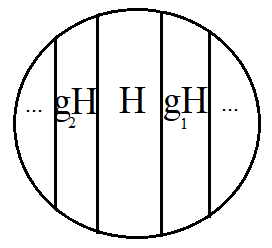
\includegraphics[width=0.75\linewidth]{Pic1}}
		\end{figure}			
		A)
		Пусть вектора $\overrightarrow{l}$, $\overrightarrow{m}$ и $\overrightarrow{n}$ такие: 
		\begin{gather*} 
			\overrightarrow{l} = \overrightarrow{KL} = \sqrt{10}\\
			\overrightarrow{m} = \overrightarrow{LM} = \sqrt{17}\\
			\overrightarrow{n} = \overrightarrow{MN} = 2\sqrt{53}
		\end{gather*}	
		Тогда: 
		\begin{gather*} 
			(\overrightarrow{l}, \overrightarrow{m}) = |\overrightarrow{l}|*|\overrightarrow{m}|*(-1*\cos\angle KLM) = \sqrt{10} * \sqrt{17} * (-1 * \frac{13}{\sqrt{170}}) = -13 \\
			(\overrightarrow{m}, \overrightarrow{n}) = |\overrightarrow{m}|*|\overrightarrow{n}|*(-1*\cos\angle LMN) = \sqrt{17} * 2\sqrt{53} * (-1 * -\frac{30}{\sqrt{901}}) = 60
		\end{gather*}
		$(\overrightarrow{l}, \overrightarrow{n}) = |\overrightarrow{l}|*|\overrightarrow{n}|*(\cos(\angle KLM + \angle LMN))$, т.к. $\overrightarrow{l} + \angle KLM = - \overrightarrow{m}$, $-\overrightarrow{m} + \angle LMN = \overrightarrow{n}$.\\ Заметим, что: 
		\begin{gather*} 
			\cos(\angle KLM + \angle LMN) = 
			\cos\angle KLM * \cos\angle LMN - \sin\angle KLM * \sin\angle LMN = \\
			\frac{13}{\sqrt{170}} * -\frac{30}{\sqrt{901}} - \frac{1}{\sqrt{170}} * \frac{1}{\sqrt{901}} = \\
			\frac{13*\sqrt{170}*(-30)*\sqrt{901}}{170*901} - \frac{1*\sqrt{170}*1*\sqrt{901}}{170*901} = \\
			\frac{-391*17\sqrt{10}\sqrt{53}}{170*901} = 
			\frac{-23*\sqrt{10}\sqrt{53}}{10*53}
		\end{gather*}
		$\sin \angle KLM * \sin \angle LMN > 0$, т.к. углы меньше $180^o$.
		\\
		\begin{gather*} 
			(\overrightarrow{l}, \overrightarrow{n}) = \overrightarrow{l} * \overrightarrow{n} * \cos(\angle KLM + \angle LMN) = \\
			\overrightarrow{l} * \overrightarrow{n} * (\cos \angle KLM * \cos \angle LMN - \sin \angle KLM * \sin \angle LMN) = \\
			\overrightarrow{l} * \overrightarrow{n} * \biggl( \cos \angle KLM * \cos \angle LMN - \sqrt{1 - (\cos \angle KLM)^2} * \sqrt{1 - (\cos \angle LMN)^2} \biggl)= \\
			\overrightarrow{KL} * \overrightarrow{MN} * \biggl( \cos \angle KLM * \cos \angle LMN - \sqrt{1 - (\cos \angle KLM)^2} * \sqrt{1 - (\cos \angle LMN)^2} \biggl)= \\
			\sqrt{10}*2*\sqrt{53}*\frac{-23*\sqrt{10}\sqrt{53}}{10*53} = -46 
		\end{gather*}
		\\	
		Найдём $(\overrightarrow{l} + \overrightarrow{m}, \overrightarrow{m} + \overrightarrow{n})$: 	
		\begin{gather*} 
			(\overrightarrow{l} + \overrightarrow{m}, \overrightarrow{m} + \overrightarrow{n}) = (\overrightarrow{l}, \overrightarrow{m}) + (\overrightarrow{l}, \overrightarrow{n}) + (\overrightarrow{m}, \overrightarrow{m}) + (\overrightarrow{m}, \overrightarrow{n}) = -13 - 46 + 17 + 60 = 18
		\end{gather*}
		\\
		С другой стороны $\alpha$ - угол между $(\overrightarrow{l} + \overrightarrow{m})$ и $(\overrightarrow{m} + \overrightarrow{n})$:
		\begin{gather*} 
			(\overrightarrow{l} + \overrightarrow{m}, \overrightarrow{m} + \overrightarrow{n}) = |\overrightarrow{l} + \overrightarrow{m}|*|\overrightarrow{m} + \overrightarrow{n}|*\cos\alpha = \\
			\sqrt{|\overrightarrow{l}|^2 + |\overrightarrow{m}|^2 - |\overrightarrow{l}|*|\overrightarrow{m}|*2*\cos\angle KLM}*\sqrt{|\overrightarrow{m}|^2 + |\overrightarrow{n}|^2 - |\overrightarrow{m}|*|\overrightarrow{n}|*2*\cos\angle LMN}*\cos\alpha = \\
			\sqrt{10 + 17 - 26}*\sqrt{17 + 212 + 120}*\cos\alpha = \sqrt{1}*\sqrt{349}*\cos\alpha
		\end{gather*}
		\\
		Откуда:
		\begin{gather*} 
			\sqrt{1}*\sqrt{349}*\cos\alpha = 18\\
			\cos\alpha = \frac{18}{\sqrt{349}} = \frac{18\sqrt{349}}{349}
		\end{gather*}	
		\\ \\
		Б)\\
		аналогично пункту (A)	
		Пусть вектора $\overrightarrow{l}$, $\overrightarrow{m}$ и $\overrightarrow{n}$ такие: 
		\begin{gather*} 
			\overrightarrow{l} = \overrightarrow{KL} = 3\sqrt{2}\\
			\overrightarrow{m} = \overrightarrow{LM} = \sqrt{13}\\
			\overrightarrow{n} = \overrightarrow{MN} = \sqrt{10}
		\end{gather*}	
		Тогда: 
		\begin{gather*} 
			(\overrightarrow{l}, \overrightarrow{m}) = |\overrightarrow{l}|*|\overrightarrow{m}|*(-1*\cos\angle KLM) = 3\sqrt{2} * \sqrt{13} * (-1 * -\frac{5}{\sqrt{26}}) = 15 \\
			(\overrightarrow{m}, \overrightarrow{n}) = |\overrightarrow{m}|*|\overrightarrow{n}|*(-1*\cos\angle LMN) = \sqrt{13} * \sqrt{10} * (-1 * -\frac{11}{\sqrt{130}}) = 11
		\end{gather*}
		$(\overrightarrow{l}, \overrightarrow{n}) = |\overrightarrow{l}|*|\overrightarrow{n}|*(\cos(\angle KLM + \angle LMN))$, т.к. $\overrightarrow{l} + \angle KLM = - \overrightarrow{m}$, $-\overrightarrow{m} + \angle LMN = \overrightarrow{n}$.\\ Заметим, что: 
		\begin{gather*} 
			\cos(\angle KLM + \angle LMN) = 
			\cos \angle KLM * \cos \angle LMN - \sin \angle KLM * \sin \angle LMN = \\
			-\frac{5}{\sqrt{26}} * -\frac{11}{\sqrt{130}} - \frac{1}{\sqrt{26}} * \frac{3}{\sqrt{130}} = \\
			\frac{(-5)*\sqrt{26}*(-11)*\sqrt{130}}{26*130} - \frac{1*\sqrt{26}*3*\sqrt{130}}{26*130} = \\
			\frac{2 \sqrt{5}}{5}
		\end{gather*}
		$\sin \angle KLM * \sin \angle LMN > 0$, т.к. углы меньше $180^\circ$.
		\\
		\begin{gather*} 
			(\overrightarrow{l}, \overrightarrow{n}) = \overrightarrow{l} * \overrightarrow{n} * \cos(\angle KLM + \angle LMN) = \\
			\overrightarrow{l} * \overrightarrow{n} * (\cos \angle KLM * \cos \angle LMN - \sin \angle KLM * \sin \angle LMN) = \\
			\overrightarrow{l} * \overrightarrow{n} * \biggl( \cos \angle KLM * \cos \angle LMN - \sqrt{1 - (\cos \angle KLM)^2} * \sqrt{1 - (\cos \angle LMN)^2} \biggl)= \\
			\overrightarrow{KL} * \overrightarrow{MN} * \biggl( \cos \angle KLM * \cos \angle LMN - \sqrt{1 - (\cos \angle KLM)^2} * \sqrt{1 - (\cos \angle LMN)^2} \biggl)= \\
			3\sqrt{2}*\sqrt{10}*\frac{2 \sqrt{5}}{5} = -12 
		\end{gather*}
		\\	
		Найдём $(\overrightarrow{l} + \overrightarrow{m}, \overrightarrow{m} + \overrightarrow{n})$: 	
		\begin{gather*} 
			(\overrightarrow{l} + \overrightarrow{m}, \overrightarrow{m} + \overrightarrow{n}) = (\overrightarrow{l}, \overrightarrow{m}) + (\overrightarrow{l}, \overrightarrow{n}) + (\overrightarrow{m}, \overrightarrow{m}) + (\overrightarrow{m}, \overrightarrow{n}) = 15 + 12 + 13 + 11 = 51
		\end{gather*}
		\\
		С другой стороны $\alpha$ - угол между $(\overrightarrow{l} + \overrightarrow{m})$ и $(\overrightarrow{m} + \overrightarrow{n})$:
		\begin{gather*} 
			(\overrightarrow{l} + \overrightarrow{m}, \overrightarrow{m} + \overrightarrow{n}) = |\overrightarrow{l} + \overrightarrow{m}|*|\overrightarrow{m} + \overrightarrow{n}|*\cos\alpha = \\
			\sqrt{|\overrightarrow{l}|^2 + |\overrightarrow{m}|^2 - |\overrightarrow{l}|*|\overrightarrow{m}|*2*\cos\angle KLM}*\sqrt{|\overrightarrow{m}|^2 + |\overrightarrow{n}|^2 - |\overrightarrow{m}|*|\overrightarrow{n}|*2*\cos\angle LMN}*\cos\alpha = \\
			\sqrt{(3\sqrt{2})^2 + (\sqrt{13})^2 - (3\sqrt{2} * \sqrt{13} * 2 * -\frac{5}{\sqrt{26}})} * \\
			\sqrt{(\sqrt{13})^2 + (\sqrt{10})^2 - (\sqrt{13} * \sqrt{10} * 2 * -\frac{11}{\sqrt{130}})}*\cos\alpha = \\
			\sqrt{18 + 13 + 30}*\sqrt{13 + 10 + 22}*\cos\alpha = \\
			\sqrt{61}*\sqrt{45}*\cos\alpha = \sqrt{61}*3\sqrt{5}*\cos\alpha
		\end{gather*}
		\\
		Откуда:
		\begin{gather*} 
			\sqrt{61}*3\sqrt{5}*\cos\alpha = 51\\
			\cos\alpha = \frac{51}{\sqrt{61} * 3\sqrt{5}} = \frac{17}{\sqrt{61} * \sqrt{5}} =\frac{17}{\sqrt{305}} = \frac{17\sqrt{305}}{305}
		\end{gather*} 
		\\ \\
		Дополнительно*)\\
		Также можно заметить, что искомый угол можно выразить напрямую из 5 входных данных(3 длин сторон и 2 углов), хотя данная форм просто является объединением всех формул, написанных выше:
		\begin{gather*} 
			\cos \angle (\overrightarrow{LN}, \overrightarrow{KM}) = \frac{(\overrightarrow{l}, \overrightarrow{m}) + (\overrightarrow{l}, \overrightarrow{n}) + (\overrightarrow{m}, \overrightarrow{m}) + (\overrightarrow{m}, \overrightarrow{n})}{|\overrightarrow{l} + \overrightarrow{m}|*|\overrightarrow{m} + \overrightarrow{n}|} = 
			\\ \\
			\frac{(\overrightarrow{l}, \overrightarrow{m}) + (\overrightarrow{l}, \overrightarrow{n}) + (\overrightarrow{m}, \overrightarrow{m}) + (\overrightarrow{m}, \overrightarrow{n})}{	\sqrt{|\overrightarrow{l}|^2 + |\overrightarrow{m}|^2 - |\overrightarrow{l}|*|\overrightarrow{m}|*2*\cos\angle KLM}*\sqrt{|\overrightarrow{m}|^2 + |\overrightarrow{n}|^2 - |\overrightarrow{m}|*|\overrightarrow{n}|*2*\cos\angle LMN}} = 
			\\ \\
			\frac{(\overrightarrow{KL}, \overrightarrow{LM}) + (\overrightarrow{KL}, \overrightarrow{MN}) + (\overrightarrow{LM}, \overrightarrow{LM}) + (\overrightarrow{LM}, \overrightarrow{MN})}{	\sqrt{|\overrightarrow{KL}|^2 + |\overrightarrow{LM}|^2 - |\overrightarrow{KL}|*|\overrightarrow{LM}|*2*\cos\angle KLM}*\sqrt{|\overrightarrow{LM}|^2 + |\overrightarrow{MN}|^2 - |\overrightarrow{LM}|*|\overrightarrow{MN}|*2*\cos\angle LMN}} = 
			\\ \\
			\frac{\overrightarrow{KL} * \overrightarrow{LM} * \cos\angle KLM}{\sqrt{|\overrightarrow{KL}|^2 + |\overrightarrow{LM}|^2 - |\overrightarrow{KL}|*|\overrightarrow{LM}|*2*\cos\angle KLM}*\sqrt{|\overrightarrow{LM}|^2 + |\overrightarrow{MN}|^2 - |\overrightarrow{LM}|*|\overrightarrow{MN}|*2*\cos\angle LMN}} + 
			\\
			\frac{\overrightarrow{KL} * \overrightarrow{MN} * \biggl( \cos \angle KLM * \cos \angle LMN - \sqrt{1 - (\cos \angle KLM)^2} * \sqrt{1 - (\cos \angle LMN)^2} \biggl)}{\sqrt{|\overrightarrow{KL}|^2 + |\overrightarrow{LM}|^2 - |\overrightarrow{KL}|*|\overrightarrow{LM}|*2*\cos\angle KLM}*\sqrt{|\overrightarrow{LM}|^2 + |\overrightarrow{MN}|^2 - |\overrightarrow{LM}|*|\overrightarrow{MN}|*2*\cos\angle LMN}} + 
			\\
			\frac{\overrightarrow{LM} * \overrightarrow{LM} * \cos{0}}{\sqrt{|\overrightarrow{KL}|^2 + |\overrightarrow{LM}|^2 - |\overrightarrow{KL}|*|\overrightarrow{LM}|*2*\cos\angle KLM}*\sqrt{|\overrightarrow{LM}|^2 + |\overrightarrow{MN}|^2 - |\overrightarrow{LM}|*|\overrightarrow{MN}|*2*\cos\angle LMN}} + 
			\\
			\frac{\overrightarrow{LM} * \overrightarrow{MN} * \cos\angle LMN}{\sqrt{|\overrightarrow{KL}|^2 + |\overrightarrow{LM}|^2 - |\overrightarrow{KL}|*|\overrightarrow{LM}|*2*\cos\angle KLM}*\sqrt{|\overrightarrow{LM}|^2 + |\overrightarrow{MN}|^2 - |\overrightarrow{LM}|*|\overrightarrow{MN}|*2*\cos\angle LMN}} 
			\\
		\end{gather*} 